\section{Progettazione}
E' stato scelto \textit{Responsive Web Design} come strategia di progettazione, il sito infatti é in grado di adattarsi graficamente in modo automatico in base al dispositivo con il quale viene visualizzato. \\
Si è preferito usare  XHTML5  perché  ci  permette  di  usare  la  specifica  WAI-ARIA descritta nella sezione x.x.x

Il progetto è stato affrontato con un approccio top-down, individuando elementi generici da implementare e procedendo quindi con lo sviluppo di pagine e funzioni.


\subsection{Struttura delle pagine}
Sono di seguito riportati i differenti elementi della struttura delle pagine del sito.
\paragraph{Header}
L' header contiene il logo ed il nome del sito, due pulsanti per visualizzare la barra di ricerca delle birre ed accedere al profilo personale oltre ad una barra di navigazione con i riferimenti alle principali pagine del sito.\\
E' presente in tutte le pagine del sito.
\paragraph{Breadcrumb}
Sotto alla testata è situata la breadcrumb che permette all'utente di orientarsi visualizzando il percorso dalla homepage fino alla pagina corrente.\\
La breadcrumb non è visibile nelle pagine di avviso di contenuto non trovato e accesso negato in quanto sono pagine di eccezione.
\paragraph{Main}
La sezione Main visualizza il contenuto principale e caratterizzante della pagina.
\paragraph{Footer}
Al piede della pagina è situato il footer che riporta informazioni sul progetto e i relativi certificati di validazione.\\
E' presente in tutte le pagine del sito.

\subsection{Struttura del sito}
L'index page del sito reindirizza alla pagina di verifica dell'età mentre conduce direttamente alla homepage se nelle variabili di sessione è inidicato che l'utente ha già eseguito la verifica ed è maggiorenne.\\
La verifica viene eseguita dalla pagina stessa \textit{ageverification} ed ogni altra pagina reindirizza a quest'ultima se rileva che nella sessione dell'utente non è presente la variabile che rappresenta l'avvenuta verifica.\\
Di seguito si riportano le pagine del sito e le rispettive caratteristiche.

\paragraph{Home}
L'homepage è la pagina che viene mostrata all'utente dopo la verifica dell'età e contiene una lista di birre in offerta o consigliate dall'amministrazione.

\paragraph{Prodotti}
La pagina \textit{prodotti} visualizza tutte le birre disponibili nel database, suddivise in pagine.\\
La pagina viene inoltre utilizzata per visualizzare i risultati di una ricerca tramite la barra di ricerca.

\paragraph{Dettagli}
La pagina \textit{dettagli} visualizza informazioni complete e recensioni della birra scelta dalla pagina Prodotti.\\
Se l'utente ha effettuato l'accesso vengono visualizzati i controlli per aggiungere e rimuovere recensioni.

\paragraph{Contatti}
La pagina \textit{contatti} contiene una breve descrizione dell'azienda ed il contatto telefonico e di posta elettronica dell'azienda.

\paragraph{Spazio utente}
La registrazione e l'accesso degli utenti viene gestita dalle pagine \textit{login} e \textit{registrazione} mentre \textit{dettagliaccount} e \textit{modificadati} permettono la visualizzazione e la modifica dei dati del proprio profilo.

\paragraph{Avvisi}
L'accesso ad aree vietate o contenuti non disponibili viene notificato dalle pagine \textit{accessdenied} e \textit{notfound} mentre il risultato di query viene visualizzato in sezioni della pagina dalla quale viene eseguita l'operazione.\\
La pagina \textit{deleteaccount} avverte della corretta eliminazione dell'account e la pagina \textit{logout} si occupa di terminare la sessione dell'utente e reindirizza alla homepage.

\subsection{Attori}
Vengono di seguito elencati i possibili tipi di utenti che possono interagire con il sito.

\paragraph{Utente non abilitato}
Se l'utente non ha una sessione attiva o ha dichiarato di essere minorenne, ogni tentativo di accesso alle pagine del sito risulta in una redirezione alla pagina di verifica dell'età, dalla quale può proseguire solo dopo aver confermato di essere maggiorenne.

\paragraph{Utente maggiorenne e non loggato}
Un utente che ha dichiarato di essere maggiorenne e non è loggato nel sito ha accesso a tutte le pagine tranne quelle di gestione dell'account; il tentativo di accesso a quest'ultime verrà negato e segnalato da una pagina apposita.
L'utente può accedere alla pagina di registrazione attraverso il link \textit{Registrati} nella pagina login, raggiungibile dal tasto account situato nell'header.
Nelle pagine di dettagli delle birre saranno visualizzate le recensioni ma non ci sarà la possibilità di modificarle o aggiungerne di nuove.


\paragraph{Utente maggiorenne e loggato}
Gli utenti che hanno effettuato l'accesso possono visitare tutte le pagine del sito ed hanno la possibilità di aggiungere ed eliminare le proprie recensioni.
Dal tasto account possono inoltre visualizzare e modificare i propri dati, effettuare il logout o eliminare l'account.

\paragraph{Utente amministratore}
Un utente amministratore ha accesso a tutte le pagine del sito e ha la possibilità di eliminare anche le recensioni degli altri utenti.
Un account deve essere eletto amministratore dagli operatori del database.

\subsection{Database}
\subsection{Accessibilità e standard}
% divisione logica/presentazione (anche formattazione testo)

\paragraph{Presentazione e CSS}
I colori dominanti del sito sono il grigio scuro e un verde pistacchio per header, sfondi e altri elementi di presentazione mentre vengono utilizzati il nero, verde e giallo per testi e link.
La palette è stata scelta in modo da garantire una corretta visualizzazione anche da persone affette da diversi tipi di cecità o sensibilità del contrasto. 


Il contenuto del sito rimane correttamente visualizzabile anche senza il caricamento dello stile CSS.

\begin{figure}[H]
	\centering
	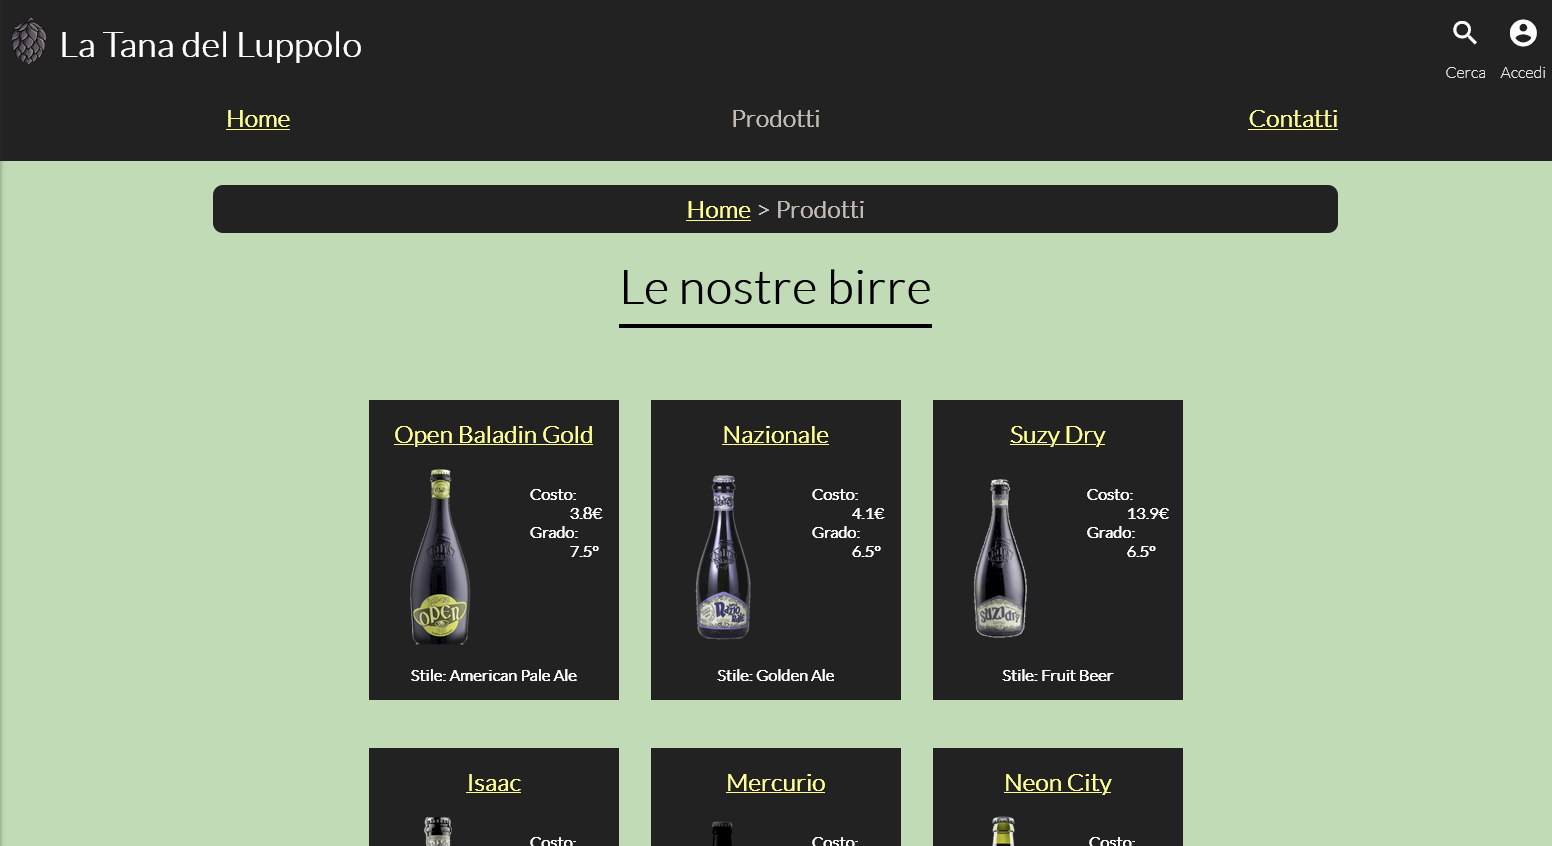
\includegraphics[width=16cm]{utility/prodotti_deuteranopia.png}
	\caption{Vista della pagina Prodotti da persone affette da deuteranopia (cecità al verde)}
\end{figure}

\paragraph{CSS di stampa}
E' stato predisposto un foglio di stile per la stampa dalla quale sono stati nascosti alcuni elementi giudicati superflui (ad esempio la barra di navigazione o i pulsanti Torna Su, ricerca e account) o modificati per migliorarne la presentazione (come la breadcrumb, le recensioni o la grandezza delle immagini principali).

\paragraph{CSS mobile}
Per i dispositivi mobili la presentazione è gestita da un apposito foglio di stile che ottimizza la visualizzazione e dispone barra di navigazione e pulsanti di ricerca e account nel menu ad hamburger nella parte destra dell'header.

\paragraph{Controlli}
I controlli sono correttamente assegnati ad una label e nelle form sono raggruppati da un tag \textit{fieldset}, descritto da un rispettivo tag \textit{legend}.


Tramite l'attributo \textit{tabindex} l'ordine di focus tramite tab viene corretto o nascosto ad alcuni elementi di presentazione, come ad esempio le icona degli utenti delle recensioni, che sono quindi marcate con il valore \textit{presentation} dell'attributo \textit{role}.


I valori provenienti dai controlli prima di essere processati lato server vengono validati e sanitizzati.

\paragraph{Altro}
% heading
% hidden link, back to top button
% lingua, charset
% alternative text
% ARIA
% label fieldset legend, gerarchia heading
% link circolari

\paragraph{Validazioni}

